%%%%%%%%%%%%%%%%%%%%%%%%%%%%%%%%%%%%%%%%%%%%%%%%%%%%%%%%%%%%
% 1.8 MODULE THEORY
% The Composition of Advanced Mathematics
%%%%%%%%%%%%%%%%%%%%%%%%%%%%%%%%%%%%%%%%%%%%%%%%%%%%%%%%%%%%

\section{Module Theory}
\label{sec:module-theory}

\prerequisite{
Linear algebra from \cref{sec:linear-algebra}, group theory from
\cref{sec:group-theory}, ring theory from \cref{sec:ring-theory}, and field
theory from \cref{sec:field-theory}.
}

\learningobjectives{
By the end of this section, the reader should be able to:
\begin{itemize}
    \item explain how modules generalize vector spaces;
    \item distinguish left modules from right modules;
    \item verify that a set with scalar multiplication is a module;
    \item recognize abelian groups as modules over \(\Z\);
    \item identify submodules and quotient modules;
    \item determine whether a subset is a submodule;
    \item work with module homomorphisms;
    \item determine kernels and images of module homomorphisms;
    \item apply the First Isomorphism Theorem for modules;
    \item understand generating sets and finitely generated modules;
    \item distinguish free modules from general modules;
    \item work with bases of free modules;
    \item understand cyclic modules;
    \item define annihilators and torsion elements;
    \item distinguish torsion and torsion-free modules;
    \item understand direct sums and decompositions;
    \item interpret ideals as modules;
    \item understand modules over quotient rings;
    \item connect linear transformations with module homomorphisms;
    \item state the structure theorem for finitely generated modules over a PID;
    \item recognize the classification of finitely generated abelian groups as a module-theoretic result.
\end{itemize}
}

%%%%%%%%%%%%%%%%%%%%%%%%%%%%%%%%%%%%%%%%%%%%%%%%%%%%%%%%%%%%
\subsection{From Vector Spaces to Modules}
\label{subsec:vector-spaces-to-modules}
%%%%%%%%%%%%%%%%%%%%%%%%%%%%%%%%%%%%%%%%%%%%%%%%%%%%%%%%%%%%

A vector space consists of vectors that can be added and multiplied by
scalars from a field.

For example,

\[ \R^n \]

is a vector space over \(\R\).

The scalar field provides powerful algebraic operations, especially division
by every nonzero scalar.

Module theory asks what happens when the scalars come from a ring instead of
a field.

\begin{conceptbox}
A module is to a ring what a vector space is to a field.

\[
\boxed{
\begin{array}{c}
\text{vector space}\\
\text{scalars from a field}
\end{array}
\quad\longrightarrow\quad
\begin{array}{c}
\text{module}\\
\text{scalars from a ring}
\end{array}}
\]
\end{conceptbox}

This seemingly small change creates a much richer theory because nonzero
elements of a ring do not necessarily possess multiplicative inverses.

%%%%%%%%%%%%%%%%%%%%%%%%%%%%%%%%%%%%%%%%%%%%%%%%%%%%%%%%%%%%
\subsection{Why Modules Matter}
\label{subsec:why-modules-matter}
%%%%%%%%%%%%%%%%%%%%%%%%%%%%%%%%%%%%%%%%%%%%%%%%%%%%%%%%%%%%

Modules provide a common language for many algebraic structures.

Examples include:

\begin{itemize}
    \item every vector space;
    \item every abelian group;
    \item every ideal of a ring;
    \item polynomial rings viewed over coefficient rings;
    \item solution spaces of linear algebraic systems;
    \item representations of groups;
    \item modules associated with linear operators;
    \item homology groups in algebraic topology.
\end{itemize}

Thus module theory connects linear algebra, group theory, ring theory,
topology, representation theory, and homological algebra.

%%%%%%%%%%%%%%%%%%%%%%%%%%%%%%%%%%%%%%%%%%%%%%%%%%%%%%%%%%%%
\subsection{Left Modules}
\label{subsec:left-modules}
%%%%%%%%%%%%%%%%%%%%%%%%%%%%%%%%%%%%%%%%%%%%%%%%%%%%%%%%%%%%

\begin{definitionbox}{Left Module}
Let \(R\) be a ring. A \emph{left \(R\)-module} is an abelian group
\((M,+)\) together with a scalar multiplication
\[ R\times M\to M,\qquad (r,m)\mapsto rm, \]
such that for all \(r,s\in R\) and \(m,n\in M\),
\[
\begin{aligned}
r(m+n)&=rm+rn,\\
(r+s)m&=rm+sm,\\
(rs)m&=r(sm),\\
1_Rm&=m
\end{aligned}
\]
when \(R\) has an identity and modules are assumed to be unital.
\end{definitionbox}

The elements of \(R\) are called \emph{scalars}, while the elements of \(M\)
are called \emph{module elements} or simply \emph{elements of the module}.

%%%%%%%%%%%%%%%%%%%%%%%%%%%%%%%%%%%%%%%%%%%%%%%%%%%%%%%%%%%%
\subsection{Visualizing the Module Structure}
\label{subsec:visual-module-structure}
%%%%%%%%%%%%%%%%%%%%%%%%%%%%%%%%%%%%%%%%%%%%%%%%%%%%%%%%%%%%

\begin{center}
\begin{tikzpicture}[
    node distance=13mm and 20mm,
    box/.style={draw,rounded corners,align=center,inner sep=6pt},
    >=stealth
]
\node[box] (R) {Ring \(R\)\\scalars};
\node[box,right=of R] (M) {Abelian group \(M\)\\module elements};
\node[box,below=of M] (M2) {New element\\\(rm\in M\)};

\draw[->,thick] (R)--node[above]{\(r\)}(M);
\draw[->,thick] (M)--node[right]{scalar action}(M2);
\draw[->,thick,bend right=35] (R) to node[left]{acts on} (M2);
\end{tikzpicture}
\end{center}

Scalar multiplication describes how the ring \(R\) acts on the additive
structure of \(M\).

%%%%%%%%%%%%%%%%%%%%%%%%%%%%%%%%%%%%%%%%%%%%%%%%%%%%%%%%%%%%
\subsection{Modules Versus Vector Spaces}
\label{subsec:modules-versus-vector-spaces}
%%%%%%%%%%%%%%%%%%%%%%%%%%%%%%%%%%%%%%%%%%%%%%%%%%%%%%%%%%%%

Every vector space is a module.

If \(F\) is a field and \(V\) is a vector space over \(F\), then \(V\) is
automatically an \(F\)-module.

The converse viewpoint is useful:

\[
\boxed{\text{vector spaces are modules over fields}.}
\]

However, modules over general rings can behave very differently.

For example, in the \(\Z\)-module \(\Z\),

\[ 2x=1 \]

has no solution in \(\Z\).

In a vector space over a field of characteristic not equal to \(2\), division
by \(2\) would be possible.

%%%%%%%%%%%%%%%%%%%%%%%%%%%%%%%%%%%%%%%%%%%%%%%%%%%%%%%%%%%%
\subsection{A Structural Comparison}
\label{subsec:module-vector-space-comparison}
%%%%%%%%%%%%%%%%%%%%%%%%%%%%%%%%%%%%%%%%%%%%%%%%%%%%%%%%%%%%

\begin{center}
\begin{tabularx}{0.9\textwidth}{@{}lXX@{}}
\toprule
& \textbf{Vector Space} & \textbf{Module}\\
\midrule
Scalars & Field \(F\) & Ring \(R\)\\
Addition & Abelian group & Abelian group\\
Scalar multiplication & Yes & Yes\\
Nonzero scalars invertible & Always & Not necessarily\\
Basis always exists & Yes & Not necessarily\\
Dimension always defined & Yes & Not generally\\
Torsion possible & No & Yes\\
\bottomrule
\end{tabularx}
\end{center}

The failure of scalar division is responsible for many of the new phenomena
in module theory.

%%%%%%%%%%%%%%%%%%%%%%%%%%%%%%%%%%%%%%%%%%%%%%%%%%%%%%%%%%%%
\subsection{Right Modules}
\label{subsec:right-modules}
%%%%%%%%%%%%%%%%%%%%%%%%%%%%%%%%%%%%%%%%%%%%%%%%%%%%%%%%%%%%

When the scalar multiplication is written

\[ M\times R\to M,\qquad(m,r)\mapsto mr, \]

the resulting structure is called a \emph{right module}.

\begin{definitionbox}{Right Module}
A \emph{right \(R\)-module} is an abelian group \(M\) equipped with a scalar
multiplication \(mr\) satisfying
\[
\begin{aligned}
(m+n)r&=mr+nr,\\
m(r+s)&=mr+ms,\\
m(rs)&=(mr)s,\\
m1_R&=m.
\end{aligned}
\]
\end{definitionbox}

If \(R\) is commutative, the distinction between left and right modules is
usually minor.

If \(R\) is noncommutative, the distinction becomes essential.

%%%%%%%%%%%%%%%%%%%%%%%%%%%%%%%%%%%%%%%%%%%%%%%%%%%%%%%%%%%%
\subsection{Bimodules}
\label{subsec:bimodules}
%%%%%%%%%%%%%%%%%%%%%%%%%%%%%%%%%%%%%%%%%%%%%%%%%%%%%%%%%%%%

A module may carry compatible scalar actions from both sides.

\begin{definitionbox}{Bimodule}
Let \(R\) and \(S\) be rings. An \((R,S)\)-\emph{bimodule} is an abelian
group \(M\) that is simultaneously a left \(R\)-module and a right
\(S\)-module such that
\[ (rm)s=r(ms) \]
for all \(r\in R\), \(s\in S\), and \(m\in M\).
\end{definitionbox}

Bimodules become particularly important in noncommutative algebra and
homological algebra.

%%%%%%%%%%%%%%%%%%%%%%%%%%%%%%%%%%%%%%%%%%%%%%%%%%%%%%%%%%%%
\subsection{First Examples of Modules}
\label{subsec:first-module-examples}
%%%%%%%%%%%%%%%%%%%%%%%%%%%%%%%%%%%%%%%%%%%%%%%%%%%%%%%%%%%%

Several familiar structures are modules.

\subsubsection{A Ring over Itself}

Every ring \(R\) is a left \(R\)-module over itself using ordinary ring
multiplication as scalar multiplication.

Thus

\[ {}_RR \]

is an \(R\)-module.

%%%%%%%%%%%%%%%%%%%%%%%%%%%%%%%%%%%%%%%%%%%%%%%%%%%%%%%%%%%%
\subsubsection{Cartesian Powers}

For any ring \(R\),

\[ R^n \]

is an \(R\)-module under componentwise addition and scalar multiplication.

If

\[ \vect{x}=(x_1,\ldots,x_n), \]

then

\[ r\vect{x}=(rx_1,\ldots,rx_n). \]

%%%%%%%%%%%%%%%%%%%%%%%%%%%%%%%%%%%%%%%%%%%%%%%%%%%%%%%%%%%%
\subsubsection{Vector Spaces}

Every vector space \(V\) over a field \(F\) is an \(F\)-module.

Thus ordinary linear algebra is contained within module theory.

%%%%%%%%%%%%%%%%%%%%%%%%%%%%%%%%%%%%%%%%%%%%%%%%%%%%%%%%%%%%
\subsubsection{Abelian Groups}

Every abelian group can be regarded as a \(\Z\)-module.

This is one of the most important examples.

%%%%%%%%%%%%%%%%%%%%%%%%%%%%%%%%%%%%%%%%%%%%%%%%%%%%%%%%%%%%
\subsection{Abelian Groups as \(\Z\)-Modules}
\label{subsec:abelian-groups-z-modules}
%%%%%%%%%%%%%%%%%%%%%%%%%%%%%%%%%%%%%%%%%%%%%%%%%%%%%%%%%%%%

Let \(A\) be an abelian group written additively.

For

\[ n\in\Z,\qquad a\in A, \]

define

\[
na=
\begin{cases}
\underbrace{a+\cdots+a}_{n\text{ times}}, & n>0,\\
0, & n=0,\\
-\underbrace{(a+\cdots+a)}_{-n\text{ times}}, & n<0.
\end{cases}
\]

This makes \(A\) into a \(\Z\)-module.

\begin{importantbox}
The study of modules over \(\Z\) is exactly the study of abelian groups.
\end{importantbox}

This connection allows results about modules to classify large classes of
abelian groups.

%%%%%%%%%%%%%%%%%%%%%%%%%%%%%%%%%%%%%%%%%%%%%%%%%%%%%%%%%%%%
\subsection{Example: \(\Z_n\) as a Module}
\label{subsec:zn-module}
%%%%%%%%%%%%%%%%%%%%%%%%%%%%%%%%%%%%%%%%%%%%%%%%%%%%%%%%%%%%

The additive group

\[ \Z/n\Z \]

is a \(\Z\)-module.

Scalar multiplication is repeated addition:

\[ k[a]=[ka]. \]

For example, in \(\Z/6\Z\),

\[ 4[2]=[8]=[2]. \]

Notice that

\[ 3[2]=[6]=[0]. \]

This illustrates a phenomenon that cannot occur in a vector space over a
field: a nonzero scalar may annihilate a nonzero module element.

%%%%%%%%%%%%%%%%%%%%%%%%%%%%%%%%%%%%%%%%%%%%%%%%%%%%%%%%%%%%
\subsection{Torsion Appears}
\label{subsec:module-torsion-preview}
%%%%%%%%%%%%%%%%%%%%%%%%%%%%%%%%%%%%%%%%%%%%%%%%%%%%%%%%%%%%

The equation

\[ 3[2]=[0] \]

in \(\Z/6\Z\) shows that module elements can be destroyed by multiplication
with nonzero scalars.

This phenomenon is called \emph{torsion}.

\begin{center}
\begin{tikzpicture}[
    node distance=14mm,
    box/.style={draw,rounded corners,inner sep=5pt},
    >=stealth
]
\node[box] (m) {\([2]\neq[0]\)};
\node[box,right=of m] (zero) {\([0]\)};
\draw[->,thick] (m)--node[above]{multiply by \(3\)}(zero);
\end{tikzpicture}
\end{center}

Torsion is one of the main reasons modules can be more complicated than
vector spaces.

%%%%%%%%%%%%%%%%%%%%%%%%%%%%%%%%%%%%%%%%%%%%%%%%%%%%%%%%%%%%
\subsection{Submodules}
\label{subsec:submodules}
%%%%%%%%%%%%%%%%%%%%%%%%%%%%%%%%%%%%%%%%%%%%%%%%%%%%%%%%%%%%

Submodules generalize vector subspaces.

\begin{definitionbox}{Submodule}
Let \(M\) be an \(R\)-module. A subset \(N\subseteq M\) is an
\emph{\(R\)-submodule} if \(N\) is itself an \(R\)-module under the operations
inherited from \(M\).
\end{definitionbox}

We write

\[ N\leq_R M \]

or simply

\[ N\leq M \]

when the scalar ring is understood.

%%%%%%%%%%%%%%%%%%%%%%%%%%%%%%%%%%%%%%%%%%%%%%%%%%%%%%%%%%%%
\subsection{The Submodule Test}
\label{subsec:submodule-test}
%%%%%%%%%%%%%%%%%%%%%%%%%%%%%%%%%%%%%%%%%%%%%%%%%%%%%%%%%%%%

\begin{theorem}[Submodule Test]
Let \(M\) be an \(R\)-module and let \(N\subseteq M\) be nonempty. Then \(N\)
is a submodule of \(M\) if for every \(x,y\in N\) and \(r\in R\),
\[ x-y\in N \]
and
\[ rx\in N. \]
\end{theorem}

Equivalently, one may verify closure under addition, additive inverses, and
scalar multiplication.

%%%%%%%%%%%%%%%%%%%%%%%%%%%%%%%%%%%%%%%%%%%%%%%%%%%%%%%%%%%%
\subsection{Example of a Submodule}
\label{subsec:submodule-example}
%%%%%%%%%%%%%%%%%%%%%%%%%%%%%%%%%%%%%%%%%%%%%%%%%%%%%%%%%%%%

Consider \(\Z\) as a \(\Z\)-module.

For any integer \(n\),

\[ n\Z=\{nk:k\in\Z\} \]

is a submodule.

For example,

\[ 6\Z\leq\Z. \]

Indeed, if

\[ a=6m,\qquad b=6n, \]

then

\[ a-b=6(m-n)\in6\Z, \]

and for every \(r\in\Z\),

\[ ra=6(rm)\in6\Z. \]

%%%%%%%%%%%%%%%%%%%%%%%%%%%%%%%%%%%%%%%%%%%%%%%%%%%%%%%%%%%%
\subsection{Ideals as Submodules}
\label{subsec:ideals-as-submodules}
%%%%%%%%%%%%%%%%%%%%%%%%%%%%%%%%%%%%%%%%%%%%%%%%%%%%%%%%%%%%

Let \(R\) be a commutative ring.

Since \(R\) is an \(R\)-module over itself, its submodules are exactly its
ideals.

Thus

\[ I\trianglelefteq R \]

can be interpreted as

\[ I\leq_R R. \]

\begin{conceptbox}
For a commutative ring \(R\),
\[ \boxed{\text{ideals of }R=\text{submodules of the module }R.} \]
\end{conceptbox}

This gives a module-theoretic interpretation of one of the central objects
from ring theory.

%%%%%%%%%%%%%%%%%%%%%%%%%%%%%%%%%%%%%%%%%%%%%%%%%%%%%%%%%%%%
\subsection{Generated Submodules}
\label{subsec:generated-submodules}
%%%%%%%%%%%%%%%%%%%%%%%%%%%%%%%%%%%%%%%%%%%%%%%%%%%%%%%%%%%%

Suppose

\[ S\subseteq M. \]

The smallest submodule of \(M\) containing \(S\) is called the submodule
generated by \(S\).

If

\[ S=\{m_1,\ldots,m_n\}, \]

then

\[ \langle m_1,\ldots,m_n\rangle \]

consists of all finite \(R\)-linear combinations

\[ r_1m_1+\cdots+r_nm_n,\qquad r_i\in R. \]

This is directly analogous to span in linear algebra.

%%%%%%%%%%%%%%%%%%%%%%%%%%%%%%%%%%%%%%%%%%%%%%%%%%%%%%%%%%%%
\subsection{Span Versus Module Generation}
\label{subsec:span-module-generation}
%%%%%%%%%%%%%%%%%%%%%%%%%%%%%%%%%%%%%%%%%%%%%%%%%%%%%%%%%%%%

In a vector space,

\[ \Span\{\vect{v}_1,\ldots,\vect{v}_n\} \]

contains all linear combinations with coefficients from a field.

In an \(R\)-module,

\[ \langle m_1,\ldots,m_n\rangle \]

contains all linear combinations with coefficients from the ring \(R\).

\begin{center}
\begin{tikzpicture}[
    node distance=11mm and 18mm,
    box/.style={draw,rounded corners,align=center,inner sep=5pt},
    >=stealth
]
\node[box] (vectors) {Generators\\\(m_1,\ldots,m_n\)};
\node[box,below left=of vectors] (ring) {Scalars\\\(r_i\in R\)};
\node[box,below right=of vectors] (comb) {Linear combinations\\\(\sum r_im_i\)};
\node[box,below=of vectors,yshift=-22mm] (module) {Generated submodule\\\(\langle m_1,\ldots,m_n\rangle\)};

\draw[->,thick] (vectors)--(comb);
\draw[->,thick] (ring)--(comb);
\draw[->,thick] (comb)--(module);
\end{tikzpicture}
\end{center}

%%%%%%%%%%%%%%%%%%%%%%%%%%%%%%%%%%%%%%%%%%%%%%%%%%%%%%%%%%%%
\subsection{Finitely Generated Modules}
\label{subsec:finitely-generated-modules}
%%%%%%%%%%%%%%%%%%%%%%%%%%%%%%%%%%%%%%%%%%%%%%%%%%%%%%%%%%%%

\begin{definitionbox}{Finitely Generated Module}
An \(R\)-module \(M\) is \emph{finitely generated} if there exist
\(m_1,\ldots,m_n\in M\) such that
\[ M=\langle m_1,\ldots,m_n\rangle. \]
\end{definitionbox}

For example,

\[ \Z^3 \]

is generated as a \(\Z\)-module by

\[ e_1=(1,0,0),\qquad e_2=(0,1,0),\qquad e_3=(0,0,1). \]

%%%%%%%%%%%%%%%%%%%%%%%%%%%%%%%%%%%%%%%%%%%%%%%%%%%%%%%%%%%%
\subsection{Cyclic Modules}
\label{subsec:cyclic-modules}
%%%%%%%%%%%%%%%%%%%%%%%%%%%%%%%%%%%%%%%%%%%%%%%%%%%%%%%%%%%%

\begin{definitionbox}{Cyclic Module}
An \(R\)-module \(M\) is \emph{cyclic} if it can be generated by a single
element:
\[ M=Rm=\{rm:r\in R\} \]
for some \(m\in M\).
\end{definitionbox}

Examples include

\[ \Z \]

as a \(\Z\)-module, generated by \(1\), and

\[ \Z/n\Z \]

as a \(\Z\)-module, generated by \([1]\).

%%%%%%%%%%%%%%%%%%%%%%%%%%%%%%%%%%%%%%%%%%%%%%%%%%%%%%%%%%%%
\subsection{Cyclic Modules and Quotient Rings}
\label{subsec:cyclic-modules-quotients}
%%%%%%%%%%%%%%%%%%%%%%%%%%%%%%%%%%%%%%%%%%%%%%%%%%%%%%%%%%%%

Suppose \(M=Rm\) is a cyclic \(R\)-module.

Consider

\[ \varphi:R\to M,\qquad\varphi(r)=rm. \]

This is a module homomorphism.

Its kernel is

\[ \Ker(\varphi)=\{r\in R:rm=0\}. \]

By the First Isomorphism Theorem,

\[ M\cong R/\Ker(\varphi). \]

Thus every cyclic module is closely related to a quotient of its scalar ring.

%%%%%%%%%%%%%%%%%%%%%%%%%%%%%%%%%%%%%%%%%%%%%%%%%%%%%%%%%%%%
\subsection{Module Homomorphisms}
\label{subsec:module-homomorphisms}
%%%%%%%%%%%%%%%%%%%%%%%%%%%%%%%%%%%%%%%%%%%%%%%%%%%%%%%%%%%%

Module homomorphisms generalize linear transformations.

\begin{definitionbox}{Module Homomorphism}
Let \(M\) and \(N\) be \(R\)-modules. A function
\[ \varphi:M\to N \]
is an \emph{\(R\)-module homomorphism} if for all \(m,n\in M\) and \(r\in R\),
\[ \varphi(m+n)=\varphi(m)+\varphi(n) \]
and
\[ \varphi(rm)=r\varphi(m). \]
\end{definitionbox}

The function must preserve both the additive structure and the scalar action.

%%%%%%%%%%%%%%%%%%%%%%%%%%%%%%%%%%%%%%%%%%%%%%%%%%%%%%%%%%%%
\subsection{Linear Transformations Are Module Homomorphisms}
\label{subsec:linear-transformations-module-homomorphisms}
%%%%%%%%%%%%%%%%%%%%%%%%%%%%%%%%%%%%%%%%%%%%%%%%%%%%%%%%%%%%

If \(V\) and \(W\) are vector spaces over a field \(F\), then an
\(F\)-module homomorphism

\[ T:V\to W \]

is exactly a linear transformation.

Thus

\[ T(a\vect{u}+b\vect{v})=aT(\vect{u})+bT(\vect{v}) \]

is the vector-space version of the module homomorphism laws.

\begin{importantbox}
Module homomorphisms generalize linear transformations from fields to
arbitrary rings.
\end{importantbox}

%%%%%%%%%%%%%%%%%%%%%%%%%%%%%%%%%%%%%%%%%%%%%%%%%%%%%%%%%%%%
\subsection{Kernel and Image}
\label{subsec:module-kernel-image}
%%%%%%%%%%%%%%%%%%%%%%%%%%%%%%%%%%%%%%%%%%%%%%%%%%%%%%%%%%%%

Let

\[ \varphi:M\to N \]

be an \(R\)-module homomorphism.

Its kernel is

\[ \Ker(\varphi)=\{m\in M:\varphi(m)=0\}. \]

Its image is

\[ \Image(\varphi)=\{\varphi(m):m\in M\}. \]

Both are submodules:

\[ \Ker(\varphi)\leq M,\qquad\Image(\varphi)\leq N. \]

%%%%%%%%%%%%%%%%%%%%%%%%%%%%%%%%%%%%%%%%%%%%%%%%%%%%%%%%%%%%
\subsection{Kernel and Image Diagram}
\label{subsec:module-kernel-image-visual}
%%%%%%%%%%%%%%%%%%%%%%%%%%%%%%%%%%%%%%%%%%%%%%%%%%%%%%%%%%%%

\begin{center}
\begin{tikzpicture}[
    node distance=28mm,
    box/.style={draw,rounded corners,minimum width=30mm,minimum height=17mm},
    >=stealth
]
\node[box] (M) {\(M\)};
\node[box,right=of M] (N) {\(N\)};

\node[below=3mm of M] {\(\Ker(\varphi)\subseteq M\)};
\node[below=3mm of N] {\(\Image(\varphi)\subseteq N\)};

\draw[->,thick] (M)--node[above]{\(\varphi\)}(N);
\end{tikzpicture}
\end{center}

The kernel measures which elements collapse to zero, while the image records
which elements are reached.

%%%%%%%%%%%%%%%%%%%%%%%%%%%%%%%%%%%%%%%%%%%%%%%%%%%%%%%%%%%%
\subsection{Worked Example: A Module Homomorphism}
\label{subsec:worked-module-homomorphism}
%%%%%%%%%%%%%%%%%%%%%%%%%%%%%%%%%%%%%%%%%%%%%%%%%%%%%%%%%%%%

\begin{workedexamplebox}{Kernel and Image of a \(\Z\)-Module Homomorphism}

Define

\[ \varphi:\Z\to\Z/6\Z,\qquad\varphi(n)=[n]. \]

Determine the kernel and image.

\begin{tabularx}{\textwidth}{@{}>{\raggedright\arraybackslash}p{0.42\textwidth}X@{}}
Find when \(\varphi(n)=[0]\). & \(n\equiv0\pmod6\)\\
Describe the kernel. & \(\Ker(\varphi)=6\Z\)\\
Determine which residue classes occur. & Every class in \(\Z/6\Z\) occurs.\\
Describe the image. & \(\Image(\varphi)=\Z/6\Z\)
\end{tabularx}

\begin{answerbox}
\[ \Ker(\varphi)=6\Z,\qquad\Image(\varphi)=\Z/6\Z. \]
\end{answerbox}
\end{workedexamplebox}

%%%%%%%%%%%%%%%%%%%%%%%%%%%%%%%%%%%%%%%%%%%%%%%%%%%%%%%%%%%%
\subsection{Module Isomorphisms}
\label{subsec:module-isomorphisms}
%%%%%%%%%%%%%%%%%%%%%%%%%%%%%%%%%%%%%%%%%%%%%%%%%%%%%%%%%%%%

\begin{definitionbox}{Module Isomorphism}
An \(R\)-module homomorphism
\[ \varphi:M\to N \]
is an \emph{isomorphism} if it is bijective.
\end{definitionbox}

If such an isomorphism exists, we write

\[ M\cong_R N \]

or simply

\[ M\cong N. \]

Isomorphic modules have the same module structure even if their elements are
represented differently.

%%%%%%%%%%%%%%%%%%%%%%%%%%%%%%%%%%%%%%%%%%%%%%%%%%%%%%%%%%%%
\subsection{Quotient Modules}
\label{subsec:quotient-modules}
%%%%%%%%%%%%%%%%%%%%%%%%%%%%%%%%%%%%%%%%%%%%%%%%%%%%%%%%%%%%

Let \(N\leq M\) be a submodule.

Since \(M\) is an abelian group under addition, we may form the quotient
group

\[ M/N. \]

Scalar multiplication is defined by

\[ r(m+N)=rm+N. \]

This turns \(M/N\) into an \(R\)-module.

\begin{definitionbox}{Quotient Module}
If \(N\leq M\) is an \(R\)-submodule, the set of cosets
\[ M/N=\{m+N:m\in M\} \]
with the induced addition and scalar multiplication is called the
\emph{quotient module}.
\end{definitionbox}

%%%%%%%%%%%%%%%%%%%%%%%%%%%%%%%%%%%%%%%%%%%%%%%%%%%%%%%%%%%%
\subsection{Visualizing a Quotient Module}
\label{subsec:quotient-module-visual}
%%%%%%%%%%%%%%%%%%%%%%%%%%%%%%%%%%%%%%%%%%%%%%%%%%%%%%%%%%%%

A quotient module treats elements differing by something in \(N\) as
equivalent.

\begin{center}
\begin{tikzpicture}[
    node distance=10mm,
    box/.style={draw,rounded corners,align=center,inner sep=5pt},
    >=stealth
]
\node[box] (M) {Module \(M\)};
\node[box,below=of M] (cosets) {Cosets\\\(m+N\)};
\node[box,below=of cosets] (Q) {Quotient module\\\(M/N\)};

\draw[->,thick] (M)--node[right]{identify modulo \(N\)}(cosets);
\draw[->,thick] (cosets)--(Q);
\end{tikzpicture}
\end{center}

%%%%%%%%%%%%%%%%%%%%%%%%%%%%%%%%%%%%%%%%%%%%%%%%%%%%%%%%%%%%
\subsection{First Isomorphism Theorem for Modules}
\label{subsec:first-isomorphism-modules}
%%%%%%%%%%%%%%%%%%%%%%%%%%%%%%%%%%%%%%%%%%%%%%%%%%%%%%%%%%%%

\begin{theorem}[First Isomorphism Theorem for Modules]
Let
\[ \varphi:M\to N \]
be an \(R\)-module homomorphism. Then
\[ M/\Ker(\varphi)\cong\Image(\varphi). \]
\end{theorem}

This is the module version of the First Isomorphism Theorems previously
encountered for groups and rings.

%%%%%%%%%%%%%%%%%%%%%%%%%%%%%%%%%%%%%%%%%%%%%%%%%%%%%%%%%%%%
\subsection{Understanding the First Isomorphism Theorem}
\label{subsec:understanding-first-module-isomorphism}
%%%%%%%%%%%%%%%%%%%%%%%%%%%%%%%%%%%%%%%%%%%%%%%%%%%%%%%%%%%%

The theorem says that the kernel contains exactly the information lost by the
homomorphism.

After collapsing the kernel,

\[ M/\Ker(\varphi), \]

the resulting quotient has exactly the same structure as the image.

\begin{center}
\begin{tikzpicture}[
    node distance=15mm and 20mm,
    box/.style={draw,rounded corners,align=center,inner sep=5pt},
    >=stealth
]
\node[box] (M) {\(M\)};
\node[box,right=of M] (I) {\(\Image(\varphi)\)};
\node[box,below=of M] (Q) {\(M/\Ker(\varphi)\)};

\draw[->,thick] (M)--node[above]{\(\varphi\)}(I);
\draw[->,thick] (M)--node[left]{quotient}(Q);
\draw[->,thick] (Q)--node[below right]{\(\cong\)}(I);
\end{tikzpicture}
\end{center}

%%%%%%%%%%%%%%%%%%%%%%%%%%%%%%%%%%%%%%%%%%%%%%%%%%%%%%%%%%%%
\subsection{Free Modules}
\label{subsec:free-modules}
%%%%%%%%%%%%%%%%%%%%%%%%%%%%%%%%%%%%%%%%%%%%%%%%%%%%%%%%%%%%

Vector spaces possess bases.

For modules, bases exist only in special cases.

\begin{definitionbox}{Free Module}
An \(R\)-module \(M\) is \emph{free} if there exists a subset
\[ B=\{b_i\}_{i\in I} \]
such that every \(m\in M\) can be written uniquely as a finite linear
combination
\[ m=\sum_{i\in I}r_ib_i,\qquad r_i\in R. \]
The set \(B\) is called a \emph{basis} of \(M\).
\end{definitionbox}

The word ``finite'' means that only finitely many coefficients \(r_i\) are
nonzero.

%%%%%%%%%%%%%%%%%%%%%%%%%%%%%%%%%%%%%%%%%%%%%%%%%%%%%%%%%%%%
\subsection{Standard Free Modules}
\label{subsec:standard-free-modules}
%%%%%%%%%%%%%%%%%%%%%%%%%%%%%%%%%%%%%%%%%%%%%%%%%%%%%%%%%%%%

The standard example is

\[ R^n. \]

Its standard basis is

\[ e_1=(1,0,\ldots,0),\quad e_2=(0,1,\ldots,0),\quad\ldots,\quad e_n=(0,\ldots,0,1). \]

Every element

\[ (r_1,\ldots,r_n)\in R^n \]

has the unique representation

\[ r_1e_1+\cdots+r_ne_n. \]

Thus \(R^n\) is a free \(R\)-module.

%%%%%%%%%%%%%%%%%%%%%%%%%%%%%%%%%%%%%%%%%%%%%%%%%%%%%%%%%%%%
\subsection{Visualizing a Free Module}
\label{subsec:free-module-visual}
%%%%%%%%%%%%%%%%%%%%%%%%%%%%%%%%%%%%%%%%%%%%%%%%%%%%%%%%%%%%

For \(R=\R\), the familiar geometry of a basis appears.

\begin{center}
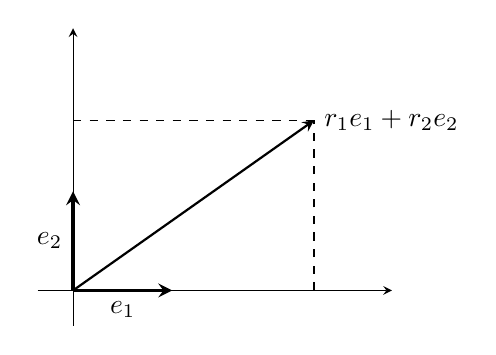
\begin{tikzpicture}[scale=0.9,>=stealth]
\draw[->] (-0.5,0)--(4.5,0);
\draw[->] (0,-0.5)--(0,3.7);

\draw[->,very thick] (0,0)--(1.4,0)
    node[midway,below]{\(e_1\)};
\draw[->,very thick] (0,0)--(0,1.4)
    node[midway,left]{\(e_2\)};

\draw[->,thick] (0,0)--(3.4,2.4)
    node[right]{\(r_1e_1+r_2e_2\)};

\draw[dashed] (3.4,0)--(3.4,2.4);
\draw[dashed] (0,2.4)--(3.4,2.4);
\end{tikzpicture}
\end{center}

For general rings, the same algebraic idea survives even when geometric
interpretation is unavailable.

%%%%%%%%%%%%%%%%%%%%%%%%%%%%%%%%%%%%%%%%%%%%%%%%%%%%%%%%%%%%
\subsection{Not Every Module Is Free}
\label{subsec:not-every-module-free}
%%%%%%%%%%%%%%%%%%%%%%%%%%%%%%%%%%%%%%%%%%%%%%%%%%%%%%%%%%%%

This is a major difference from vector spaces.

Consider

\[ \Z/2\Z \]

as a \(\Z\)-module.

Suppose it had a basis containing a nonzero element \(m\).

Then

\[ 2m=0. \]

Thus the expression

\[ 0m \]

and the expression

\[ 2m \]

would represent the same element using different coefficients.

This violates uniqueness.

Therefore,

\[ \Z/2\Z \]

is not a free \(\Z\)-module.

\begin{warningbox}
Every vector space has a basis, but not every module has a basis.
\end{warningbox}

%%%%%%%%%%%%%%%%%%%%%%%%%%%%%%%%%%%%%%%%%%%%%%%%%%%%%%%%%%%%
\subsection{Rank of a Free Module}
\label{subsec:rank-free-module}
%%%%%%%%%%%%%%%%%%%%%%%%%%%%%%%%%%%%%%%%%%%%%%%%%%%%%%%%%%%%

For many important rings, especially commutative rings satisfying suitable
conditions, bases of a finite-rank free module have the same number of
elements.

\begin{definitionbox}{Rank of a Free Module}
If a free \(R\)-module \(M\) has a finite basis
\[ \{b_1,\ldots,b_n\}, \]
then its \emph{rank} is
\[ \rank_R(M)=n. \]
\end{definitionbox}

For example,

\[ \rank_R(R^n)=n. \]

This generalizes dimension from linear algebra.

%%%%%%%%%%%%%%%%%%%%%%%%%%%%%%%%%%%%%%%%%%%%%%%%%%%%%%%%%%%%
\subsection{Linear Independence in Modules}
\label{subsec:module-linear-independence}
%%%%%%%%%%%%%%%%%%%%%%%%%%%%%%%%%%%%%%%%%%%%%%%%%%%%%%%%%%%%

Elements

\[ m_1,\ldots,m_n\in M \]

are \emph{linearly independent over \(R\)} if

\[ r_1m_1+\cdots+r_nm_n=0 \]

implies

\[ r_1=\cdots=r_n=0. \]

This looks identical to the vector-space definition.

However, the behavior can be very different because \(R\) may contain zero
divisors or noninvertible elements.

%%%%%%%%%%%%%%%%%%%%%%%%%%%%%%%%%%%%%%%%%%%%%%%%%%%%%%%%%%%%
\subsection{Example of Failed Independence}
\label{subsec:failed-module-independence}
%%%%%%%%%%%%%%%%%%%%%%%%%%%%%%%%%%%%%%%%%%%%%%%%%%%%%%%%%%%%

Consider

\[ M=\Z/6\Z \]

as a \(\Z\)-module.

The element

\[ [2]\neq[0] \]

does not form a linearly independent set because

\[ 3[2]=[0] \]

while

\[ 3\neq0 \]

in \(\Z\).

Thus nonzero elements need not behave like nonzero vectors in a vector space.

%%%%%%%%%%%%%%%%%%%%%%%%%%%%%%%%%%%%%%%%%%%%%%%%%%%%%%%%%%%%
\subsection{Annihilators}
\label{subsec:annihilators}
%%%%%%%%%%%%%%%%%%%%%%%%%%%%%%%%%%%%%%%%%%%%%%%%%%%%%%%%%%%%

\begin{definitionbox}{Annihilator of an Element}
Let \(M\) be an \(R\)-module and \(m\in M\). The \emph{annihilator} of \(m\)
is
\[ \Ann_R(m)=\{r\in R:rm=0\}. \]
\end{definitionbox}

The notation

\[ \Ann_R(m) \]

is read ``the annihilator of \(m\) in \(R\).''

For a commutative ring \(R\), \(\Ann_R(m)\) is an ideal of \(R\).

%%%%%%%%%%%%%%%%%%%%%%%%%%%%%%%%%%%%%%%%%%%%%%%%%%%%%%%%%%%%
\subsection{Example of an Annihilator}
\label{subsec:annihilator-example}
%%%%%%%%%%%%%%%%%%%%%%%%%%%%%%%%%%%%%%%%%%%%%%%%%%%%%%%%%%%%

Consider

\[ [2]\in\Z/6\Z. \]

We seek all integers \(n\) satisfying

\[ n[2]=[0]. \]

This occurs exactly when

\[ 6\mid2n, \]

or equivalently,

\[ 3\mid n. \]

Therefore,

\[ \Ann_{\Z}([2])=3\Z. \]

%%%%%%%%%%%%%%%%%%%%%%%%%%%%%%%%%%%%%%%%%%%%%%%%%%%%%%%%%%%%
\subsection{Annihilator of a Module}
\label{subsec:annihilator-module}
%%%%%%%%%%%%%%%%%%%%%%%%%%%%%%%%%%%%%%%%%%%%%%%%%%%%%%%%%%%%

\begin{definitionbox}{Annihilator of a Module}
The \emph{annihilator} of an \(R\)-module \(M\) is
\[ \Ann_R(M)=\{r\in R:rm=0\text{ for every }m\in M\}. \]
\end{definitionbox}

Equivalently,

\[ \Ann_R(M)=\bigcap_{m\in M}\Ann_R(m). \]

%%%%%%%%%%%%%%%%%%%%%%%%%%%%%%%%%%%%%%%%%%%%%%%%%%%%%%%%%%%%
\subsection{Torsion Elements}
\label{subsec:torsion-elements}
%%%%%%%%%%%%%%%%%%%%%%%%%%%%%%%%%%%%%%%%%%%%%%%%%%%%%%%%%%%%

Suppose \(R\) is an integral domain.

\begin{definitionbox}{Torsion Element}
An element \(m\in M\) is a \emph{torsion element} if there exists a nonzero
\(r\in R\) such that
\[ rm=0. \]
\end{definitionbox}

The zero element is always torsion.

A nonzero torsion element is therefore an element annihilated by some nonzero
scalar.

%%%%%%%%%%%%%%%%%%%%%%%%%%%%%%%%%%%%%%%%%%%%%%%%%%%%%%%%%%%%
\subsection{The Torsion Submodule}
\label{subsec:torsion-submodule}
%%%%%%%%%%%%%%%%%%%%%%%%%%%%%%%%%%%%%%%%%%%%%%%%%%%%%%%%%%%%

For a module \(M\) over an integral domain \(R\), define

\[ T(M)=\{m\in M:rm=0\text{ for some nonzero }r\in R\}. \]

Under these assumptions, \(T(M)\) is a submodule of \(M\), called the
\emph{torsion submodule}.

%%%%%%%%%%%%%%%%%%%%%%%%%%%%%%%%%%%%%%%%%%%%%%%%%%%%%%%%%%%%
\subsection{Torsion and Torsion-Free Modules}
\label{subsec:torsion-free-modules}
%%%%%%%%%%%%%%%%%%%%%%%%%%%%%%%%%%%%%%%%%%%%%%%%%%%%%%%%%%%%

\begin{definitionbox}{Torsion Module}
An \(R\)-module \(M\) is a \emph{torsion module} if every element of \(M\) is
a torsion element.
\end{definitionbox}

\begin{definitionbox}{Torsion-Free Module}
An \(R\)-module \(M\) is \emph{torsion-free} if
\[ rm=0,\qquad r\neq0 \]
implies
\[ m=0. \]
\end{definitionbox}

For example,

\[ \Z \]

is torsion-free as a \(\Z\)-module, while

\[ \Z/n\Z \]

is a torsion \(\Z\)-module.

%%%%%%%%%%%%%%%%%%%%%%%%%%%%%%%%%%%%%%%%%%%%%%%%%%%%%%%%%%%%
\subsection{Torsion as an Obstruction to Freeness}
\label{subsec:torsion-obstruction-free}
%%%%%%%%%%%%%%%%%%%%%%%%%%%%%%%%%%%%%%%%%%%%%%%%%%%%%%%%%%%%

If \(R\) is an integral domain, every free \(R\)-module is torsion-free.

Indeed, suppose

\[ M=R^n \]

and

\[ r\vect{x}=\zero \]

with \(r\neq0\).

Since \(R\) has no zero divisors,

\[ \vect{x}=\zero. \]

Therefore a module containing nonzero torsion cannot be free over an integral
domain.

%%%%%%%%%%%%%%%%%%%%%%%%%%%%%%%%%%%%%%%%%%%%%%%%%%%%%%%%%%%%
\subsection{Direct Sums of Modules}
\label{subsec:direct-sums-modules}
%%%%%%%%%%%%%%%%%%%%%%%%%%%%%%%%%%%%%%%%%%%%%%%%%%%%%%%%%%%%

Let \(M\) and \(N\) be \(R\)-modules.

Their direct sum is

\[ M\oplus N=\{(m,n):m\in M,\ n\in N\}, \]

with operations defined componentwise:

\[ (m_1,n_1)+(m_2,n_2)=(m_1+m_2,n_1+n_2), \]

and

\[ r(m,n)=(rm,rn). \]

The symbol

\[ \oplus \]

is read ``direct sum.''

%%%%%%%%%%%%%%%%%%%%%%%%%%%%%%%%%%%%%%%%%%%%%%%%%%%%%%%%%%%%
\subsection{Internal Direct Sums}
\label{subsec:internal-direct-sums}
%%%%%%%%%%%%%%%%%%%%%%%%%%%%%%%%%%%%%%%%%%%%%%%%%%%%%%%%%%%%

Suppose \(A,B\leq M\).

If

\[ M=A+B \]

and

\[ A\cap B=\{0\}, \]

then

\[ M=A\oplus B. \]

Every element \(m\in M\) then has a unique representation

\[ m=a+b,\qquad a\in A,\quad b\in B. \]

%%%%%%%%%%%%%%%%%%%%%%%%%%%%%%%%%%%%%%%%%%%%%%%%%%%%%%%%%%%%
\subsection{Visualizing a Direct Sum}
\label{subsec:direct-sum-visual}
%%%%%%%%%%%%%%%%%%%%%%%%%%%%%%%%%%%%%%%%%%%%%%%%%%%%%%%%%%%%

In \(\R^2\),

\[ \R^2=\Span\{e_1\}\oplus\Span\{e_2\}. \]

\begin{center}
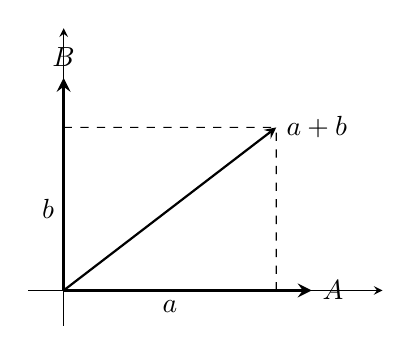
\begin{tikzpicture}[scale=0.9,>=stealth]
\draw[->] (-0.5,0)--(4.5,0);
\draw[->] (0,-0.5)--(0,3.7);

\draw[->,very thick] (0,0)--(3.5,0)
    node[right]{\(A\)};
\draw[->,very thick] (0,0)--(0,3)
    node[above]{\(B\)};

\coordinate (P) at (3,2.3);
\draw[->,thick] (0,0)--(P)
    node[right]{\(a+b\)};
\draw[dashed] (3,0)--(P);
\draw[dashed] (0,2.3)--(P);

\node[below] at (1.5,0) {\(a\)};
\node[left] at (0,1.15) {\(b\)};
\end{tikzpicture}
\end{center}

The vector-space picture is a special geometric case of the general
module-theoretic decomposition.

%%%%%%%%%%%%%%%%%%%%%%%%%%%%%%%%%%%%%%%%%%%%%%%%%%%%%%%%%%%%
\subsection{Direct Summands}
\label{subsec:direct-summands}
%%%%%%%%%%%%%%%%%%%%%%%%%%%%%%%%%%%%%%%%%%%%%%%%%%%%%%%%%%%%

\begin{definitionbox}{Direct Summand}
A submodule \(N\leq M\) is a \emph{direct summand} if there exists another
submodule \(P\leq M\) such that
\[ M=N\oplus P. \]
\end{definitionbox}

The module \(P\) is called a complement of \(N\).

Not every submodule has a complement.

This is another important contrast with finite-dimensional vector spaces.

%%%%%%%%%%%%%%%%%%%%%%%%%%%%%%%%%%%%%%%%%%%%%%%%%%%%%%%%%%%%
\subsection{Module Endomorphisms}
\label{subsec:module-endomorphisms}
%%%%%%%%%%%%%%%%%%%%%%%%%%%%%%%%%%%%%%%%%%%%%%%%%%%%%%%%%%%%

An \(R\)-module homomorphism

\[ \varphi:M\to M \]

is called an \emph{endomorphism}.

The set of all endomorphisms of \(M\) is denoted

\[ \End_R(M). \]

Addition is defined pointwise:

\[ (\varphi+\psi)(m)=\varphi(m)+\psi(m), \]

and multiplication is composition:

\[ (\varphi\psi)(m)=\varphi(\psi(m)). \]

Under these operations,

\[ \End_R(M) \]

forms a ring.

%%%%%%%%%%%%%%%%%%%%%%%%%%%%%%%%%%%%%%%%%%%%%%%%%%%%%%%%%%%%
\subsection{Matrices as Module Homomorphisms}
\label{subsec:matrices-module-homomorphisms}
%%%%%%%%%%%%%%%%%%%%%%%%%%%%%%%%%%%%%%%%%%%%%%%%%%%%%%%%%%%%

Let \(R\) be a commutative ring.

An \(m\times n\) matrix

\[ A\in M_{m\times n}(R) \]

defines an \(R\)-module homomorphism

\[ T_A:R^n\to R^m \]

by

\[ T_A(\vect{x})=A\vect{x}. \]

Thus matrix algebra extends naturally from vector spaces to free modules.

\begin{center}
\begin{tikzpicture}[
    node distance=25mm,
    box/.style={draw,rounded corners,minimum width=25mm,minimum height=10mm},
    >=stealth
]
\node[box] (Rn) {\(R^n\)};
\node[box,right=of Rn] (Rm) {\(R^m\)};
\draw[->,thick] (Rn)--node[above]{\(A\)}node[below]{\(\vect{x}\mapsto A\vect{x}\)}(Rm);
\end{tikzpicture}
\end{center}

%%%%%%%%%%%%%%%%%%%%%%%%%%%%%%%%%%%%%%%%%%%%%%%%%%%%%%%%%%%%
\subsection{Modules over Polynomial Rings}
\label{subsec:modules-polynomial-rings}
%%%%%%%%%%%%%%%%%%%%%%%%%%%%%%%%%%%%%%%%%%%%%%%%%%%%%%%%%%%%

One of the most powerful connections with linear algebra comes from
polynomial rings.

Let \(V\) be a vector space over a field \(F\), and let

\[ T:V\to V \]

be a linear transformation.

We can make \(V\) into an \(F[x]\)-module by defining

\[ f(x)\cdot\vect{v}=f(T)(\vect{v}). \]

In particular,

\[ x\cdot\vect{v}=T(\vect{v}). \]

Thus the indeterminate \(x\) acts as the linear operator \(T\).

%%%%%%%%%%%%%%%%%%%%%%%%%%%%%%%%%%%%%%%%%%%%%%%%%%%%%%%%%%%%
\subsection{Visualizing the Polynomial Action}
\label{subsec:polynomial-module-action-visual}
%%%%%%%%%%%%%%%%%%%%%%%%%%%%%%%%%%%%%%%%%%%%%%%%%%%%%%%%%%%%

\begin{center}
\begin{tikzpicture}[
    node distance=13mm,
    box/.style={draw,rounded corners,align=center,inner sep=5pt},
    >=stealth
]
\node[box] (x) {Polynomial scalar\\\(x\in F[x]\)};
\node[box,below=of x] (T) {Linear operator\\\(T\)};
\node[box,below=of T] (v) {Vector\\\(\vect{v}\)};
\node[box,below=of v] (Tv) {Result\\\(T(\vect{v})\)};

\draw[->,thick] (x)--node[right]{acts as}(T);
\draw[->,thick] (T)--(v);
\draw[->,thick] (v)--(Tv);
\end{tikzpicture}
\end{center}

More generally,

\[ (a_0+a_1x+\cdots+a_nx^n)\cdot\vect{v}
=a_0\vect{v}+a_1T\vect{v}+\cdots+a_nT^n\vect{v}. \]

%%%%%%%%%%%%%%%%%%%%%%%%%%%%%%%%%%%%%%%%%%%%%%%%%%%%%%%%%%%%
\subsection{Invariant Subspaces as Submodules}
\label{subsec:invariant-subspaces-submodules}
%%%%%%%%%%%%%%%%%%%%%%%%%%%%%%%%%%%%%%%%%%%%%%%%%%%%%%%%%%%%

Under the \(F[x]\)-module structure induced by \(T\), a subspace

\[ W\subseteq V \]

is an \(F[x]\)-submodule precisely when

\[ T(W)\subseteq W. \]

Thus invariant subspaces from linear algebra are exactly submodules in this
module structure.

This reveals that much of linear operator theory can be reinterpreted as
module theory.

%%%%%%%%%%%%%%%%%%%%%%%%%%%%%%%%%%%%%%%%%%%%%%%%%%%%%%%%%%%%
\subsection{Annihilating Polynomials}
\label{subsec:annihilating-polynomials}
%%%%%%%%%%%%%%%%%%%%%%%%%%%%%%%%%%%%%%%%%%%%%%%%%%%%%%%%%%%%

Suppose \(V\) is viewed as an \(F[x]\)-module through a linear operator \(T\).

A polynomial

\[ f(x)\in F[x] \]

annihilates \(\vect{v}\in V\) if

\[ f(T)(\vect{v})=\zero. \]

A polynomial annihilates all of \(V\) if

\[ f(T)=0. \]

The minimal polynomial of \(T\) is therefore naturally connected with the
annihilator ideal of the \(F[x]\)-module \(V\).

%%%%%%%%%%%%%%%%%%%%%%%%%%%%%%%%%%%%%%%%%%%%%%%%%%%%%%%%%%%%
\subsection{Modules over Quotient Rings}
\label{subsec:modules-quotient-rings}
%%%%%%%%%%%%%%%%%%%%%%%%%%%%%%%%%%%%%%%%%%%%%%%%%%%%%%%%%%%%

Suppose an ideal \(I\trianglelefteq R\) annihilates an \(R\)-module \(M\):

\[ IM=0. \]

Then the scalar action depends only on residue classes modulo \(I\).

Consequently, \(M\) can naturally be regarded as an \(R/I\)-module.

For example,

\[ \Z/n\Z \]

is naturally a module over the quotient ring

\[ \Z/n\Z. \]

%%%%%%%%%%%%%%%%%%%%%%%%%%%%%%%%%%%%%%%%%%%%%%%%%%%%%%%%%%%%
\subsection{Exact Sequences: A First Look}
\label{subsec:module-exact-sequences}
%%%%%%%%%%%%%%%%%%%%%%%%%%%%%%%%%%%%%%%%%%%%%%%%%%%%%%%%%%%%

Module homomorphisms are often organized into sequences.

Consider

\[ A\xrightarrow{f}B\xrightarrow{g}C. \]

\begin{definitionbox}{Exactness}
The sequence
\[ A\xrightarrow{f}B\xrightarrow{g}C \]
is \emph{exact at \(B\)} if
\[ \Image(f)=\Ker(g). \]
\end{definitionbox}

Exactness says that everything produced by one map is exactly what is
destroyed by the next map.

%%%%%%%%%%%%%%%%%%%%%%%%%%%%%%%%%%%%%%%%%%%%%%%%%%%%%%%%%%%%
\subsection{Short Exact Sequences}
\label{subsec:short-exact-sequences}
%%%%%%%%%%%%%%%%%%%%%%%%%%%%%%%%%%%%%%%%%%%%%%%%%%%%%%%%%%%%

A sequence

\[ 0\longrightarrow A\xrightarrow{f}B\xrightarrow{g}C\longrightarrow0 \]

is called a \emph{short exact sequence} if it is exact at every position.

This implies:

\begin{itemize}
    \item \(f\) is injective;
    \item \(g\) is surjective;
    \item \(\Image(f)=\Ker(g)\).
\end{itemize}

\begin{center}
\begin{tikzpicture}[
    node distance=12mm,
    every node/.style={font=\small},
    >=stealth
]
\node (z1) {\(0\)};
\node[right=of z1] (A) {\(A\)};
\node[right=of A] (B) {\(B\)};
\node[right=of B] (C) {\(C\)};
\node[right=of C] (z2) {\(0\)};

\draw[->,thick] (z1)--(A);
\draw[->,thick] (A)--node[above]{\(f\)}(B);
\draw[->,thick] (B)--node[above]{\(g\)}(C);
\draw[->,thick] (C)--(z2);
\end{tikzpicture}
\end{center}

Exact sequences become a central language of homological algebra.

%%%%%%%%%%%%%%%%%%%%%%%%%%%%%%%%%%%%%%%%%%%%%%%%%%%%%%%%%%%%
\subsection{A Standard Short Exact Sequence}
\label{subsec:standard-short-exact-sequence}
%%%%%%%%%%%%%%%%%%%%%%%%%%%%%%%%%%%%%%%%%%%%%%%%%%%%%%%%%%%%

If \(N\leq M\), then

\[ 0\longrightarrow N\xrightarrow{\iota}M\xrightarrow{\pi}M/N\longrightarrow0 \]

is exact.

Here

\[ \iota(n)=n \]

is the inclusion map, and

\[ \pi(m)=m+N \]

is the quotient map.

Since

\[ \Ker(\pi)=N=\Image(\iota), \]

the sequence is exact.

%%%%%%%%%%%%%%%%%%%%%%%%%%%%%%%%%%%%%%%%%%%%%%%%%%%%%%%%%%%%
\subsection{Splitting}
\label{subsec:module-splitting}
%%%%%%%%%%%%%%%%%%%%%%%%%%%%%%%%%%%%%%%%%%%%%%%%%%%%%%%%%%%%

A short exact sequence

\[ 0\to A\to B\to C\to0 \]

is said to \emph{split} when \(B\) decomposes, under suitable equivalent
conditions, as

\[ B\cong A\oplus C. \]

Thus splitting converts an extension into a direct-sum decomposition.

The deeper theory of exact sequences and splitting will be developed
canonically in homological algebra.

%%%%%%%%%%%%%%%%%%%%%%%%%%%%%%%%%%%%%%%%%%%%%%%%%%%%%%%%%%%%
\subsection{Modules over Principal Ideal Domains}
\label{subsec:modules-pids}
%%%%%%%%%%%%%%%%%%%%%%%%%%%%%%%%%%%%%%%%%%%%%%%%%%%%%%%%%%%%

Module theory becomes especially well behaved over a principal ideal domain,
or PID.

Important examples include

\[ \Z \]

and

\[ F[x] \]

when \(F\) is a field.

Because every ideal in a PID is generated by one element, finitely generated
modules over PIDs admit a powerful classification theorem.

%%%%%%%%%%%%%%%%%%%%%%%%%%%%%%%%%%%%%%%%%%%%%%%%%%%%%%%%%%%%
\subsection{Structure Theorem over a PID}
\label{subsec:structure-theorem-pid}
%%%%%%%%%%%%%%%%%%%%%%%%%%%%%%%%%%%%%%%%%%%%%%%%%%%%%%%%%%%%

\begin{theorem}[Structure Theorem for Finitely Generated Modules over a PID]
Let \(R\) be a principal ideal domain and let \(M\) be a finitely generated
\(R\)-module. Then
\[ M\cong R^r\oplus R/(d_1)\oplus\cdots\oplus R/(d_k), \]
where
\[ d_1\mid d_2\mid\cdots\mid d_k \]
and each \(d_i\neq0\) is a nonunit.
\end{theorem}

The notation

\[ d_1\mid d_2 \]

is read ``\(d_1\) divides \(d_2\).''

The component

\[ R^r \]

is the free part of the module, while the quotient modules form the torsion
part.

%%%%%%%%%%%%%%%%%%%%%%%%%%%%%%%%%%%%%%%%%%%%%%%%%%%%%%%%%%%%
\subsection{Visualizing the Structure Theorem}
\label{subsec:structure-theorem-visual}
%%%%%%%%%%%%%%%%%%%%%%%%%%%%%%%%%%%%%%%%%%%%%%%%%%%%%%%%%%%%

\begin{center}
\begin{tikzpicture}[
    node distance=12mm and 18mm,
    box/.style={draw,rounded corners,align=center,inner sep=6pt},
    >=stealth
]
\node[box] (M) {Finitely generated\\module \(M\) over a PID};
\node[box,below left=of M] (free) {Free part\\\(R^r\)};
\node[box,below right=of M] (torsion) {Torsion part\\\(\bigoplus_iR/(d_i)\)};

\draw[->,thick] (M)--(free);
\draw[->,thick] (M)--(torsion);

\node[below=10mm of M] {\(\displaystyle M\cong R^r\oplus\bigoplus_iR/(d_i)\)};
\end{tikzpicture}
\end{center}

This decomposition is analogous to breaking a complicated object into basic
building blocks.

%%%%%%%%%%%%%%%%%%%%%%%%%%%%%%%%%%%%%%%%%%%%%%%%%%%%%%%%%%%%
\subsection{Invariant Factors}
\label{subsec:module-invariant-factors}
%%%%%%%%%%%%%%%%%%%%%%%%%%%%%%%%%%%%%%%%%%%%%%%%%%%%%%%%%%%%

In the decomposition

\[ M\cong R^r\oplus R/(d_1)\oplus\cdots\oplus R/(d_k), \]

with

\[ d_1\mid d_2\mid\cdots\mid d_k, \]

the elements \(d_i\) are called \emph{invariant factors}.

Up to multiplication by units, these factors are uniquely determined by the
module.

They therefore serve as algebraic invariants.

%%%%%%%%%%%%%%%%%%%%%%%%%%%%%%%%%%%%%%%%%%%%%%%%%%%%%%%%%%%%
\subsection{Elementary Divisors}
\label{subsec:module-elementary-divisors}
%%%%%%%%%%%%%%%%%%%%%%%%%%%%%%%%%%%%%%%%%%%%%%%%%%%%%%%%%%%%

The torsion part may alternatively be decomposed using powers of irreducible
elements.

Schematically,

\[ M_{\text{tors}}\cong\bigoplus_iR/(p_i^{\,k_i}). \]

These powers are called the \emph{elementary divisors} of the module.

The invariant-factor and elementary-divisor forms encode equivalent
classification information in different arrangements.

%%%%%%%%%%%%%%%%%%%%%%%%%%%%%%%%%%%%%%%%%%%%%%%%%%%%%%%%%%%%
\subsection{Classification of Finitely Generated Abelian Groups}
\label{subsec:fg-abelian-groups-modules}
%%%%%%%%%%%%%%%%%%%%%%%%%%%%%%%%%%%%%%%%%%%%%%%%%%%%%%%%%%%%

Take

\[ R=\Z. \]

Since \(\Z\) is a PID, the structure theorem applies to finitely generated
\(\Z\)-modules.

But \(\Z\)-modules are exactly abelian groups.

Therefore every finitely generated abelian group has the form

\[ G\cong\Z^r\oplus\Z/d_1\Z\oplus\cdots\oplus\Z/d_k\Z, \]

where

\[ d_1\mid d_2\mid\cdots\mid d_k. \]

Thus the classification theorem for finitely generated abelian groups is a
special case of module theory.

%%%%%%%%%%%%%%%%%%%%%%%%%%%%%%%%%%%%%%%%%%%%%%%%%%%%%%%%%%%%
\subsection{Example of Abelian Group Decomposition}
\label{subsec:abelian-group-decomposition-example}
%%%%%%%%%%%%%%%%%%%%%%%%%%%%%%%%%%%%%%%%%%%%%%%%%%%%%%%%%%%%

Consider

\[ G=\Z^2\oplus\Z/4\Z\oplus\Z/12\Z. \]

The free part is

\[ \Z^2, \]

so the free rank is \(2\).

The torsion part is

\[ \Z/4\Z\oplus\Z/12\Z. \]

Because

\[ 4\mid12, \]

this is already in invariant-factor form.

%%%%%%%%%%%%%%%%%%%%%%%%%%%%%%%%%%%%%%%%%%%%%%%%%%%%%%%%%%%%
\subsection{Worked Example: Free and Torsion Parts}
\label{subsec:worked-free-torsion-parts}
%%%%%%%%%%%%%%%%%%%%%%%%%%%%%%%%%%%%%%%%%%%%%%%%%%%%%%%%%%%%

\begin{workedexamplebox}{Identifying Free and Torsion Components}

Consider the \(\Z\)-module

\[ M=\Z^3\oplus\Z/6\Z\oplus\Z/30\Z. \]

Identify its free rank and torsion submodule.

\begin{tabularx}{\textwidth}{@{}>{\raggedright\arraybackslash}p{0.42\textwidth}X@{}}
Identify the free component. & \(\Z^3\)\\
Read the free rank. & \(r=3\)\\
Identify finite cyclic components. & \(\Z/6\Z,\ \Z/30\Z\)\\
Combine them as the torsion part. & \(T(M)=\Z/6\Z\oplus\Z/30\Z\)
\end{tabularx}

\begin{answerbox}
\[ \rank_{\Z}(M)=3,\qquad T(M)\cong\Z/6\Z\oplus\Z/30\Z. \]
\end{answerbox}
\end{workedexamplebox}

%%%%%%%%%%%%%%%%%%%%%%%%%%%%%%%%%%%%%%%%%%%%%%%%%%%%%%%%%%%%
\subsection{Connection with Smith Normal Form}
\label{subsec:smith-normal-form-modules}
%%%%%%%%%%%%%%%%%%%%%%%%%%%%%%%%%%%%%%%%%%%%%%%%%%%%%%%%%%%%

Matrices over a PID can often be simplified using invertible row and column
operations.

The resulting canonical form is called the \emph{Smith normal form}.

For a matrix \(A\), the Smith normal form has the schematic shape

\[
D=
\begin{bmatrix}
d_1 & 0 & \cdots & 0\\
0 & d_2 & \cdots & 0\\
\vdots & \vdots & \ddots & \vdots\\
0 & 0 & \cdots & d_r
\end{bmatrix},
\]

where

\[ d_1\mid d_2\mid\cdots\mid d_r. \]

These diagonal entries encode invariant factors of associated modules.

%%%%%%%%%%%%%%%%%%%%%%%%%%%%%%%%%%%%%%%%%%%%%%%%%%%%%%%%%%%%
\subsection{A Module Presented by Generators and Relations}
\label{subsec:module-presentations}
%%%%%%%%%%%%%%%%%%%%%%%%%%%%%%%%%%%%%%%%%%%%%%%%%%%%%%%%%%%%

A finitely generated module can often be described by generators together
with relations.

For example, suppose \(M\) is generated by

\[ x_1,\ldots,x_n \]

subject to relations encoded by a matrix \(A\).

This gives a presentation

\[ R^m\xrightarrow{A}R^n\longrightarrow M\longrightarrow0. \]

Equivalently,

\[ M\cong R^n/\Image(A). \]

This viewpoint makes matrices central to the classification of modules.

%%%%%%%%%%%%%%%%%%%%%%%%%%%%%%%%%%%%%%%%%%%%%%%%%%%%%%%%%%%%
\subsection{Generators, Relations, and Quotients}
\label{subsec:generators-relations-visual}
%%%%%%%%%%%%%%%%%%%%%%%%%%%%%%%%%%%%%%%%%%%%%%%%%%%%%%%%%%%%

\begin{center}
\begin{tikzpicture}[
    node distance=12mm,
    box/.style={draw,rounded corners,align=center,inner sep=5pt},
    >=stealth
]
\node[box] (free) {Free module\\\(R^n\)};
\node[box,below=of free] (relations) {Relations\\\(\Image(A)\)};
\node[box,below=of relations] (quotient) {Presented module\\\(R^n/\Image(A)\)};

\draw[->,thick] (free)--(relations);
\draw[->,thick] (relations)--node[right]{quotient}(quotient);
\end{tikzpicture}
\end{center}

The free module provides independent generators; quotienting by the relation
submodule imposes the desired algebraic relations.

%%%%%%%%%%%%%%%%%%%%%%%%%%%%%%%%%%%%%%%%%%%%%%%%%%%%%%%%%%%%
\subsection{Example: A Cyclic Presentation}
\label{subsec:cyclic-presentation-example}
%%%%%%%%%%%%%%%%%%%%%%%%%%%%%%%%%%%%%%%%%%%%%%%%%%%%%%%%%%%%

Consider a \(\Z\)-module generated by \(x\) subject to the relation

\[ 6x=0. \]

The free module on one generator is

\[ \Z. \]

The relation generates the submodule

\[ 6\Z. \]

Therefore,

\[ M\cong\Z/6\Z. \]

Thus the familiar cyclic group \(\Z/6\Z\) can be viewed as one generator
subject to one relation.

%%%%%%%%%%%%%%%%%%%%%%%%%%%%%%%%%%%%%%%%%%%%%%%%%%%%%%%%%%%%
\subsection{Modules and Canonical Forms in Linear Algebra}
\label{subsec:modules-canonical-linear-algebra}
%%%%%%%%%%%%%%%%%%%%%%%%%%%%%%%%%%%%%%%%%%%%%%%%%%%%%%%%%%%%

Let \(V\) be a finite-dimensional vector space over \(F\), equipped with a
linear operator

\[ T:V\to V. \]

Viewing \(V\) as an \(F[x]\)-module transforms the classification of linear
operators into the classification of finitely generated modules over the PID

\[ F[x]. \]

This leads to canonical matrix forms such as:

\begin{itemize}
    \item rational canonical form;
    \item companion matrices;
    \item invariant factors;
    \item elementary divisors;
    \item Jordan canonical form when the relevant polynomials split.
\end{itemize}

Thus module theory explains why these canonical forms exist.

%%%%%%%%%%%%%%%%%%%%%%%%%%%%%%%%%%%%%%%%%%%%%%%%%%%%%%%%%%%%
\subsection{The Structural Relationship}
\label{subsec:module-linear-operator-structure}
%%%%%%%%%%%%%%%%%%%%%%%%%%%%%%%%%%%%%%%%%%%%%%%%%%%%%%%%%%%%

\begin{center}
\begin{tikzpicture}[
    node distance=11mm,
    box/.style={draw,rounded corners,align=center,inner sep=5pt},
    >=stealth
]
\node[box] (T) {Linear operator\\\(T:V\to V\)};
\node[box,below=of T] (module) {\(F[x]\)-module\\structure on \(V\)};
\node[box,below=of module] (structure) {PID module\\structure theorem};
\node[box,below left=of structure] (inv) {Invariant factors};
\node[box,below right=of structure] (canon) {Canonical matrix\\forms};

\draw[->,thick] (T)--(module);
\draw[->,thick] (module)--(structure);
\draw[->,thick] (structure)--(inv);
\draw[->,thick] (structure)--(canon);
\end{tikzpicture}
\end{center}

This is a major example of how abstract algebra explains concrete linear
algebra.

%%%%%%%%%%%%%%%%%%%%%%%%%%%%%%%%%%%%%%%%%%%%%%%%%%%%%%%%%%%%
\subsection{Simple Modules}
\label{subsec:simple-modules}
%%%%%%%%%%%%%%%%%%%%%%%%%%%%%%%%%%%%%%%%%%%%%%%%%%%%%%%%%%%%

\begin{definitionbox}{Simple Module}
A nonzero \(R\)-module \(M\) is \emph{simple} if its only submodules are
\[ \{0\}\qquad\text{and}\qquad M. \]
\end{definitionbox}

Simple modules are module-theoretic analogues of irreducible building blocks.

For example, if \(F\) is a field, then \(F\) is a simple \(F\)-module.

%%%%%%%%%%%%%%%%%%%%%%%%%%%%%%%%%%%%%%%%%%%%%%%%%%%%%%%%%%%%
\subsection{Simple \(\Z\)-Modules}
\label{subsec:simple-z-modules}
%%%%%%%%%%%%%%%%%%%%%%%%%%%%%%%%%%%%%%%%%%%%%%%%%%%%%%%%%%%%

The simple \(\Z\)-modules are precisely

\[ \Z/p\Z \]

where \(p\) is prime.

Indeed, the submodules of \(\Z/p\Z\) correspond to its additive subgroups.

Since a cyclic group of prime order has no nontrivial proper subgroup,
\(\Z/p\Z\) is simple.

%%%%%%%%%%%%%%%%%%%%%%%%%%%%%%%%%%%%%%%%%%%%%%%%%%%%%%%%%%%%
\subsection{Maximal Ideals and Simple Modules}
\label{subsec:maximal-ideals-simple-modules}
%%%%%%%%%%%%%%%%%%%%%%%%%%%%%%%%%%%%%%%%%%%%%%%%%%%%%%%%%%%%

Let \(R\) be a commutative ring with identity and let
\(\mathfrak m\) be a maximal ideal.

Then

\[ R/\mathfrak m \]

is a field.

As an \(R\)-module,

\[ R/\mathfrak m \]

is simple.

Conversely, every simple cyclic \(R\)-module is isomorphic to

\[ R/\mathfrak m \]

for some maximal ideal \(\mathfrak m\).

This connects simple modules with maximal ideals.

%%%%%%%%%%%%%%%%%%%%%%%%%%%%%%%%%%%%%%%%%%%%%%%%%%%%%%%%%%%%
\subsection{Noetherian Modules}
\label{subsec:noetherian-modules}
%%%%%%%%%%%%%%%%%%%%%%%%%%%%%%%%%%%%%%%%%%%%%%%%%%%%%%%%%%%%

Module theory also provides a natural framework for finiteness conditions.

\begin{definitionbox}{Noetherian Module}
An \(R\)-module \(M\) is \emph{Noetherian} if every ascending chain of
submodules
\[ M_1\subseteq M_2\subseteq M_3\subseteq\cdots \]
eventually stabilizes.
\end{definitionbox}

That is, there exists \(N\) such that

\[ M_N=M_{N+1}=M_{N+2}=\cdots. \]

Equivalent formulations include the condition that every submodule of \(M\)
is finitely generated.

%%%%%%%%%%%%%%%%%%%%%%%%%%%%%%%%%%%%%%%%%%%%%%%%%%%%%%%%%%%%
\subsection{Ascending Chain Condition}
\label{subsec:ascending-chain-condition-modules}
%%%%%%%%%%%%%%%%%%%%%%%%%%%%%%%%%%%%%%%%%%%%%%%%%%%%%%%%%%%%

The stabilization property is called the \emph{ascending chain condition},
abbreviated ACC.

\begin{center}
\begin{tikzpicture}[
    node distance=8mm,
    every node/.style={font=\small},
    >=stealth
]
\node (M1) {\(M_1\)};
\node[right=of M1] (M2) {\(M_2\)};
\node[right=of M2] (M3) {\(M_3\)};
\node[right=of M3] (MN) {\(M_N\)};
\node[right=of MN] (same1) {\(M_N\)};
\node[right=of same1] (same2) {\(\cdots\)};

\draw[->] (M1)--node[above]{\(\subseteq\)}(M2);
\draw[->] (M2)--node[above]{\(\subseteq\)}(M3);
\draw[->,dashed] (M3)--(MN);
\draw[->] (MN)--node[above]{\(=\)}(same1);
\draw[->] (same1)--node[above]{\(=\)}(same2);
\end{tikzpicture}
\end{center}

%%%%%%%%%%%%%%%%%%%%%%%%%%%%%%%%%%%%%%%%%%%%%%%%%%%%%%%%%%%%
\subsection{Artinian Modules}
\label{subsec:artinian-modules}
%%%%%%%%%%%%%%%%%%%%%%%%%%%%%%%%%%%%%%%%%%%%%%%%%%%%%%%%%%%%

The dual descending condition gives another important class.

\begin{definitionbox}{Artinian Module}
An \(R\)-module \(M\) is \emph{Artinian} if every descending chain
\[ M_1\supseteq M_2\supseteq M_3\supseteq\cdots \]
eventually stabilizes.
\end{definitionbox}

This is called the \emph{descending chain condition}, abbreviated DCC.

Noetherian and Artinian conditions become especially important in
commutative algebra and representation theory.

%%%%%%%%%%%%%%%%%%%%%%%%%%%%%%%%%%%%%%%%%%%%%%%%%%%%%%%%%%%%
\subsection{Modules as Representations}
\label{subsec:modules-as-representations}
%%%%%%%%%%%%%%%%%%%%%%%%%%%%%%%%%%%%%%%%%%%%%%%%%%%%%%%%%%%%

Suppose a group \(G\) acts linearly on a vector space \(V\) over a field
\(F\).

This action can be encoded using the group algebra

\[ F[G]. \]

Then \(V\) becomes an \(F[G]\)-module.

Consequently,

\[
\boxed{
\text{linear representations of }G
\longleftrightarrow
F[G]\text{-modules}.
}
\]

This connection forms one of the foundations of representation theory.

%%%%%%%%%%%%%%%%%%%%%%%%%%%%%%%%%%%%%%%%%%%%%%%%%%%%%%%%%%%%
\subsection{Modules in Algebraic Topology}
\label{subsec:modules-algebraic-topology}
%%%%%%%%%%%%%%%%%%%%%%%%%%%%%%%%%%%%%%%%%%%%%%%%%%%%%%%%%%%%

Homology groups arising in algebraic topology are abelian groups and
therefore \(\Z\)-modules.

For example,

\[ H_n(X;\Z) \]

is a \(\Z\)-module.

The structure theorem for finitely generated modules over \(\Z\) therefore
helps classify homology groups of many topological spaces.

This is an important example of algebraic structure being used to describe
geometric and topological objects.

%%%%%%%%%%%%%%%%%%%%%%%%%%%%%%%%%%%%%%%%%%%%%%%%%%%%%%%%%%%%
\subsection{Modules in Homological Algebra}
\label{subsec:modules-homological-algebra}
%%%%%%%%%%%%%%%%%%%%%%%%%%%%%%%%%%%%%%%%%%%%%%%%%%%%%%%%%%%%

Module categories provide the standard setting for homological algebra.

Important constructions include:

\begin{itemize}
    \item exact sequences;
    \item projective modules;
    \item injective modules;
    \item tensor products;
    \item \(\operatorname{Hom}\) modules;
    \item chain complexes;
    \item derived functors;
    \item \(\operatorname{Tor}\);
    \item \(\operatorname{Ext}\).
\end{itemize}

These topics will be developed canonically in
\cref{sec:homological-algebra} rather than duplicated here.

%%%%%%%%%%%%%%%%%%%%%%%%%%%%%%%%%%%%%%%%%%%%%%%%%%%%%%%%%%%%
\subsection{Common Errors in Module Theory}
\label{subsec:common-module-errors}
%%%%%%%%%%%%%%%%%%%%%%%%%%%%%%%%%%%%%%%%%%%%%%%%%%%%%%%%%%%%

\subsubsection{Assuming Every Module Is a Vector Space}

A vector space requires scalars from a field.

A module may use scalars from a general ring.

For example,

\[ \Z \]

is a \(\Z\)-module but not a vector space over \(\Z\), because \(\Z\) is not
a field.

%%%%%%%%%%%%%%%%%%%%%%%%%%%%%%%%%%%%%%%%%%%%%%%%%%%%%%%%%%%%
\subsubsection{Assuming Every Module Has a Basis}

Modules need not be free.

For example,

\[ \Z/2\Z \]

has no basis as a \(\Z\)-module.

%%%%%%%%%%%%%%%%%%%%%%%%%%%%%%%%%%%%%%%%%%%%%%%%%%%%%%%%%%%%
\subsubsection{Assuming Every Submodule Has a Complement}

In vector spaces, every subspace has a complementary subspace.

For general modules this may fail.

Thus

\[ N\leq M \]

does not automatically imply

\[ M=N\oplus P \]

for some submodule \(P\).

%%%%%%%%%%%%%%%%%%%%%%%%%%%%%%%%%%%%%%%%%%%%%%%%%%%%%%%%%%%%
\subsubsection{Ignoring Left and Right Scalar Actions}

For a noncommutative ring,

\[ rm \]

and

\[ mr \]

belong to different module structures.

One cannot interchange left and right modules without justification.

%%%%%%%%%%%%%%%%%%%%%%%%%%%%%%%%%%%%%%%%%%%%%%%%%%%%%%%%%%%%
\subsubsection{Treating Torsion Like Linear Dependence over a Field}

In modules, a nonzero scalar can sometimes annihilate a nonzero element:

\[ rm=0,\qquad r\neq0,\quad m\neq0. \]

This cannot occur in a vector space over a field.

%%%%%%%%%%%%%%%%%%%%%%%%%%%%%%%%%%%%%%%%%%%%%%%%%%%%%%%%%%%%
\subsubsection{Confusing Ideals and Arbitrary Submodules}

Ideals are submodules of a ring viewed as a module over itself.

Submodules of an arbitrary module are not themselves ideals unless additional
structure makes that statement meaningful.

%%%%%%%%%%%%%%%%%%%%%%%%%%%%%%%%%%%%%%%%%%%%%%%%%%%%%%%%%%%%
\subsubsection{Assuming Rank Behaves Exactly Like Dimension}

Dimension is universally well behaved for vector spaces.

Module rank requires more care and depends on properties of the scalar ring
and the module.

%%%%%%%%%%%%%%%%%%%%%%%%%%%%%%%%%%%%%%%%%%%%%%%%%%%%%%%%%%%%
\subsubsection{Confusing Direct Sum with Ordinary Sum}

The condition

\[ M=A+B \]

does not by itself imply

\[ M=A\oplus B. \]

For an internal direct sum, one also requires

\[ A\cap B=\{0\}. \]

%%%%%%%%%%%%%%%%%%%%%%%%%%%%%%%%%%%%%%%%%%%%%%%%%%%%%%%%%%%%
\subsection{Applications of Module Theory}
\label{subsec:module-theory-applications}
%%%%%%%%%%%%%%%%%%%%%%%%%%%%%%%%%%%%%%%%%%%%%%%%%%%%%%%%%%%%

\begin{applicationbox}
\textbf{Linear Algebra.}
Vector spaces are modules over fields, and linear transformations are module
homomorphisms. Modules over \(F[x]\) explain invariant subspaces, minimal
polynomials, and canonical matrix forms.

\medskip

\textbf{Abelian Groups.}
Abelian groups are precisely \(\Z\)-modules. Their classification is a
special case of the structure theorem for finitely generated modules over a
PID.

\medskip

\textbf{Ring Theory.}
Ideals are submodules of a ring over itself. Modules provide a natural way to
study how rings act on other algebraic objects.

\medskip

\textbf{Representation Theory.}
Linear representations of a group \(G\) over a field \(F\) can be studied as
modules over the group algebra \(F[G]\).

\medskip

\textbf{Algebraic Topology.}
Homology groups are modules, and module decompositions reveal algebraic
information about topological spaces.

\medskip

\textbf{Commutative Algebra.}
Noetherian modules, localization, tensor products, and finitely generated
modules are fundamental tools in the study of commutative rings.

\medskip

\textbf{Homological Algebra.}
Exact sequences and module homomorphisms provide the basic language for
projective resolutions, derived functors, \(\operatorname{Tor}\), and
\(\operatorname{Ext}\).

\medskip

\textbf{Algebraic Geometry.}
Modules over coordinate rings correspond to algebraic and geometric
structures and eventually lead to sheaves and coherent sheaves.
\end{applicationbox}

%%%%%%%%%%%%%%%%%%%%%%%%%%%%%%%%%%%%%%%%%%%%%%%%%%%%%%%%%%%%
\subsection{Structural Map of Module Theory}
\label{subsec:module-theory-structural-map}
%%%%%%%%%%%%%%%%%%%%%%%%%%%%%%%%%%%%%%%%%%%%%%%%%%%%%%%%%%%%

\begin{center}
\begin{tikzpicture}[
    node distance=9mm and 13mm,
    box/.style={draw,rounded corners,align=center,inner sep=4pt,font=\small},
    >=stealth
]
\node[box] (module) {\(R\)-module};
\node[box,below left=of module] (sub) {Submodules};
\node[box,below right=of module] (hom) {Homomorphisms};

\node[box,below=of sub] (quot) {Quotient modules};
\node[box,below=of hom] (ker) {Kernel and image};

\node[box,below left=of quot] (free) {Free modules};
\node[box,below right=of quot] (torsion) {Torsion};

\node[box,below left=of ker] (direct) {Direct sums};
\node[box,below right=of ker] (exact) {Exact sequences};

\node[box,below=25mm of torsion] (pid) {Modules over PIDs};
\node[box,below=of pid] (structure) {Structure theorem};

\draw[->] (module)--(sub);
\draw[->] (module)--(hom);
\draw[->] (sub)--(quot);
\draw[->] (hom)--(ker);
\draw[->] (quot)--(free);
\draw[->] (quot)--(torsion);
\draw[->] (ker)--(direct);
\draw[->] (ker)--(exact);
\draw[->] (free)--(pid);
\draw[->] (torsion)--(pid);
\draw[->] (pid)--(structure);
\end{tikzpicture}
\end{center}

%%%%%%%%%%%%%%%%%%%%%%%%%%%%%%%%%%%%%%%%%%%%%%%%%%%%%%%%%%%%
\subsection{Exercises}
\label{subsec:module-theory-exercises}
%%%%%%%%%%%%%%%%%%%%%%%%%%%%%%%%%%%%%%%%%%%%%%%%%%%%%%%%%%%%

\begin{exercise}[1]
Explain the difference between a vector space and a module.
\end{exercise}

\begin{exercise}[1]
Why is every vector space a module?
\end{exercise}

\begin{exercise}[1]
Explain why every abelian group is naturally a \(\Z\)-module.
\end{exercise}

\begin{exercise}[1]
Show that \(\Z^2\) is a \(\Z\)-module under componentwise operations.
\end{exercise}

\begin{exercise}[1]
Show that \(\Z/8\Z\) is a \(\Z\)-module.
\end{exercise}

\begin{exercise}[2]
Verify all module axioms for \(R^n\) as an \(R\)-module.
\end{exercise}

\begin{exercise}[1]
Determine whether
\[ 4\Z \]
is a submodule of \(\Z\) as a \(\Z\)-module.
\end{exercise}

\begin{exercise}[2]
Show that every ideal of a commutative ring \(R\) is an \(R\)-submodule of
\(R\).
\end{exercise}

\begin{exercise}[2]
Show that every \(R\)-submodule of \(R\) is an ideal when \(R\) is
commutative.
\end{exercise}

\begin{exercise}[1]
Find the submodule of \(\Z\) generated by \(12\).
\end{exercise}

\begin{exercise}[2]
Find the submodule of \(\Z\) generated by \(12\) and \(18\).
\end{exercise}

\begin{exercise}[1]
Determine whether \(\Z\) is cyclic as a \(\Z\)-module.
\end{exercise}

\begin{exercise}[1]
Determine whether \(\Z^2\) is cyclic as a \(\Z\)-module.
\end{exercise}

\begin{exercise}[2]
Show that every cyclic \(R\)-module is isomorphic to \(R/I\) for some ideal
\(I\) when \(R\) is commutative.
\end{exercise}

\begin{exercise}[2]
Define
\[ \varphi:\Z\to\Z/10\Z,\qquad\varphi(n)=[n]. \]
Find \(\Ker(\varphi)\) and \(\Image(\varphi)\).
\end{exercise}

\begin{exercise}[2]
Use the First Isomorphism Theorem to prove
\[ \Z/10\Z\cong\Image(\varphi) \]
for the previous exercise.
\end{exercise}

\begin{exercise}[2]
Show that the kernel of a module homomorphism is a submodule.
\end{exercise}

\begin{exercise}[2]
Show that the image of a module homomorphism is a submodule.
\end{exercise}

\begin{exercise}[2]
Show that the composition of two \(R\)-module homomorphisms is an
\(R\)-module homomorphism.
\end{exercise}

\begin{exercise}[1]
Show that \(R^3\) is a free \(R\)-module.
\end{exercise}

\begin{exercise}[1]
Find a standard basis for \(R^4\).
\end{exercise}

\begin{exercise}[2]
Explain why \(\Z/5\Z\) is not a free \(\Z\)-module.
\end{exercise}

\begin{exercise}[2]
Prove that a free module over an integral domain is torsion-free.
\end{exercise}

\begin{exercise}[1]
Find
\[ \Ann_{\Z}([3]) \]
where \([3]\in\Z/12\Z\).
\end{exercise}

\begin{exercise}[2]
Find
\[ \Ann_{\Z}([4]) \]
where \([4]\in\Z/18\Z\).
\end{exercise}

\begin{exercise}[1]
Determine the torsion elements of \(\Z\).
\end{exercise}

\begin{exercise}[1]
Determine the torsion elements of \(\Z/12\Z\).
\end{exercise}

\begin{exercise}[2]
Determine the torsion submodule of
\[ \Z^2\oplus\Z/6\Z. \]
\end{exercise}

\begin{exercise}[2]
Show that
\[ \Z^2=\Z(1,0)\oplus\Z(0,1). \]
\end{exercise}

\begin{exercise}[2]
Let
\[ A=\Z(1,0),\qquad B=\Z(1,2)\subseteq\Z^2. \]
Determine whether
\[ \Z^2=A\oplus B. \]
\end{exercise}

\begin{exercise}[2]
Explain why not every submodule of a module must be a direct summand.
\end{exercise}

\begin{exercise}[2]
Show that
\[ \End_R(M) \]
forms a ring under pointwise addition and composition.
\end{exercise}

\begin{exercise}[2]
Let \(A\in M_{2\times2}(\Z)\). Show that
\[ T_A:\Z^2\to\Z^2,\qquad T_A(\vect{x})=A\vect{x} \]
is a \(\Z\)-module homomorphism.
\end{exercise}

\begin{exercise}[2]
Let \(T:V\to V\) be a linear transformation over \(F\). Verify that defining
\[ x\cdot\vect{v}=T(\vect{v}) \]
extends to an \(F[x]\)-module structure on \(V\).
\end{exercise}

\begin{exercise}[2]
Show that a subspace \(W\subseteq V\) is an \(F[x]\)-submodule under the
previous construction exactly when
\[ T(W)\subseteq W. \]
\end{exercise}

\begin{exercise}[2]
For the sequence
\[ 0\to N\to M\to M/N\to0, \]
identify the inclusion and quotient maps and verify exactness.
\end{exercise}

\begin{exercise}[2]
Explain what it means for a short exact sequence to split.
\end{exercise}

\begin{exercise}[1]
Identify the free part and torsion part of
\[ \Z^4\oplus\Z/3\Z\oplus\Z/15\Z. \]
\end{exercise}

\begin{exercise}[2]
Determine the rank of
\[ \Z^5\oplus\Z/8\Z. \]
\end{exercise}

\begin{exercise}[2]
Determine whether
\[ \Z/4\Z\oplus\Z/20\Z \]
is written in invariant-factor form.
\end{exercise}

\begin{exercise}[3]
Express
\[ \Z/12\Z \]
as a direct sum of its prime-power components.
\end{exercise}

\begin{exercise}[3]
Express
\[ \Z/60\Z \]
as a direct sum of cyclic groups of prime-power order.
\end{exercise}

\begin{exercise}[2]
Explain why the classification of finitely generated abelian groups follows
from the structure theorem for finitely generated modules over a PID.
\end{exercise}

\begin{exercise}[2]
Explain the relationship between Smith normal form and module
presentations.
\end{exercise}

\begin{exercise}[2]
Describe the \(\Z\)-module with one generator \(x\) and relation
\[ 8x=0. \]
\end{exercise}

\begin{exercise}[3]
Describe the module presented by
\[ \Z\xrightarrow{\times 12}\Z\to M\to0. \]
\end{exercise}

\begin{exercise}[2]
Determine whether \(\Z/p\Z\) is a simple \(\Z\)-module when \(p\) is prime.
\end{exercise}

\begin{exercise}[2]
Explain why
\[ R/\mathfrak m \]
is a simple \(R\)-module when \(\mathfrak m\) is maximal.
\end{exercise}

\begin{exercise}[2]
State the ascending chain condition for modules.
\end{exercise}

\begin{exercise}[2]
State the descending chain condition for modules.
\end{exercise}

\begin{exercise}[3]
Explain how a representation of a group \(G\) over \(F\) can be interpreted
as an \(F[G]\)-module.
\end{exercise}

%%%%%%%%%%%%%%%%%%%%%%%%%%%%%%%%%%%%%%%%%%%%%%%%%%%%%%%%%%%%
\subsection{Section Connections}
\label{subsec:module-theory-connections}
%%%%%%%%%%%%%%%%%%%%%%%%%%%%%%%%%%%%%%%%%%%%%%%%%%%%%%%%%%%%

\chapterconnection{
Module theory extends the central ideas of \cref{sec:linear-algebra} from
vector spaces over fields to algebraic systems whose scalars come from rings.
The ring structures developed in \cref{sec:ring-theory} provide the scalar
actions, while abelian groups from \cref{sec:group-theory} provide the
underlying additive structure. Ideals become submodules of rings, linear
transformations become module homomorphisms, and quotient constructions
continue the structural patterns seen throughout algebra. Modules over PIDs
lead to classification theorems for finitely generated abelian groups and
canonical forms in linear algebra. Module theory also provides foundational
language for commutative algebra, representation theory, and homological
algebra.
}

%%%%%%%%%%%%%%%%%%%%%%%%%%%%%%%%%%%%%%%%%%%%%%%%%%%%%%%%%%%%
% SECTION SOURCE TRACKING
%%%%%%%%%%%%%%%%%%%%%%%%%%%%%%%%%%%%%%%%%%%%%%%%%%%%%%%%%%%%

%------------------------------------------------------------
% 1.8 Module Theory
%------------------------------------------------------------
%
% Sources:
%   - T. Y. Lam, A First Course in Noncommutative Rings.
%     Key: lam2001noncommutative
%
% Used for:
%   - module definitions and scalar actions;
%   - left and right module distinctions;
%   - submodules and module homomorphisms;
%   - cyclic and free modules;
%   - annihilators and module structure;
%   - module-theoretic perspective connecting rings and linear algebra.
%
% Notes:
%   - Vector-space foundations are treated canonically in Section 1.2.
%   - Group foundations are treated canonically in Section 1.4.
%   - Ring and ideal foundations are treated canonically in Section 1.5.
%   - Field foundations are treated canonically in Section 1.6.
%   - Exact sequences are introduced only at the level needed to motivate
%     later homological algebra.
%   - Detailed projective, injective, flat, tensor, Hom, Tor, and Ext theory
%     belongs to Section 1.13, Homological Algebra.
%   - Noetherian module theory is developed further in Section 1.9,
%     Commutative Algebra.
%   - Representation-theoretic module structures are developed further in
%     Section 1.11, Representation Theory.
%   - Visualizations and exposition are independently developed for this text.
%
\nocite{lam2001noncommutative}